%Section comment: There seem to be missing terms near lines 20-21.
\section{Summary of Paper \ref{pap:daiyong}}
\subsection*{"\nameref{pap:daiyong}"}
The Least Square Support Vector Regression (LS-SVR) \cite{brereton_support_2010} is used in Paper \ref{pap:daiyong} to identify the parameters in the AVMM.  
The source of the data is experimental tests using a ship model in a lake with a scale of 50:1. The configuration of sensors and equipment used for the experiment are displayed in \autoref{fig:cthmodel}.  
\begin{figure}[H]
    \centering
    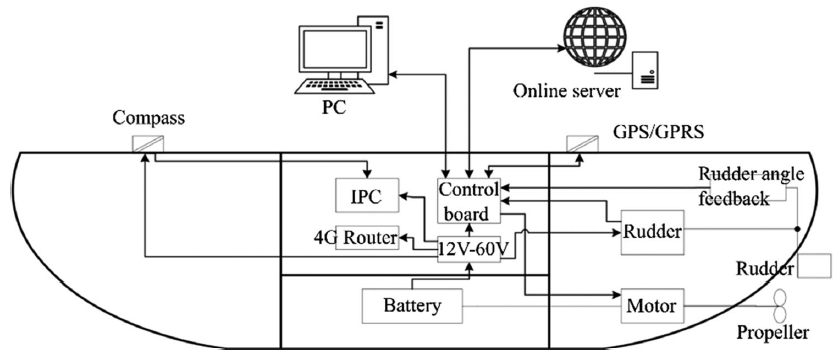
\includegraphics[width=\textwidth]{kappa/images/cth_model.png}
    \caption{Configuration of sensors and equipment for the experimental tests.}
    \label{fig:cthmodel}
\end{figure}
\noindent The hydrodynamic derivatives of the AVMM are identified almost flawlessly when applied to data from simulations with the MSS toolbox Mariner \cite{tristan_matlab_2009}. It is not effective when applied to the data obtained from the lake experiments, as seen in \autoref{fig:daiyong_extrapolation}. 

\begin{figure}[H]
    \centering
    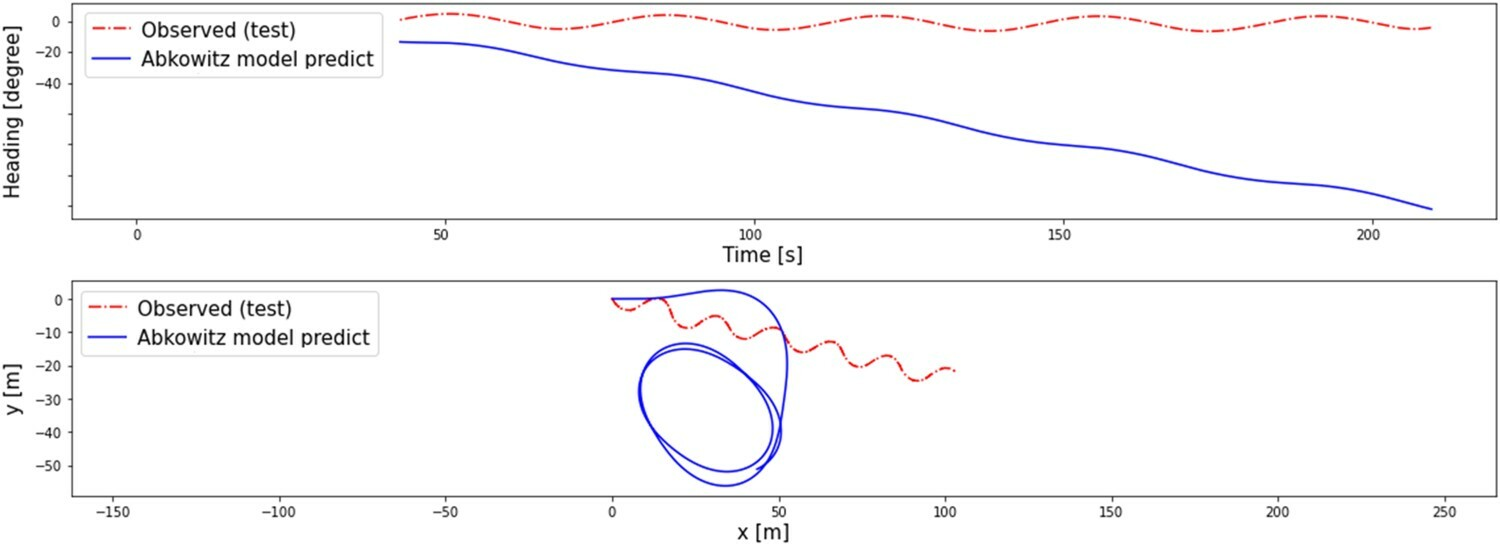
\includegraphics[width=\linewidth]{kappa/images/daiyong_extrapolation.jpeg}
    \caption{Prediction with AVMM of zigzag lake experiments.}
    \label{fig:daiyong_extrapolation}
\end{figure}

\noindent The parameter estimation is very sensitive to noise due to the differentiation that is required to calculate velocities and yaw rate from the measured position and heading. The parameter estimation is more effective if the data is first cleansed using a proposed preprocessing algorithm along with a Kalman filter (KF). The simulations with the identified model and the experiments still did not agree very much.